\section{ \ac{BLE} beacons}
\label{sec:beacon}


The beacons that were utilized are Texas Instruments CC2650STK devices which can be visualized in figure ~\ref{fig:beacon}. Alongside the device, which comes with a pre-installed bluetooth low energy program capable of giving information on each of its ten sensors through its predefined profiles, there is a texas smartphone application that can connect to a single device and read from its sensors. By using the texas Code Composer Studio (CSS), the pre-defined ble profile existant on the device could be altered. Upon further analysis of the profile, a characteristic was found for which the Universal Unique Identifier (UUID) of the service and the characteristic itself was found and as such this was the one that ended up being used to store the device's owner server's address. Since the device was already set to work as a pheripheral and it now stored the information relevant to the system, there was no need to do further work.

\begin{figure}
	\centering
		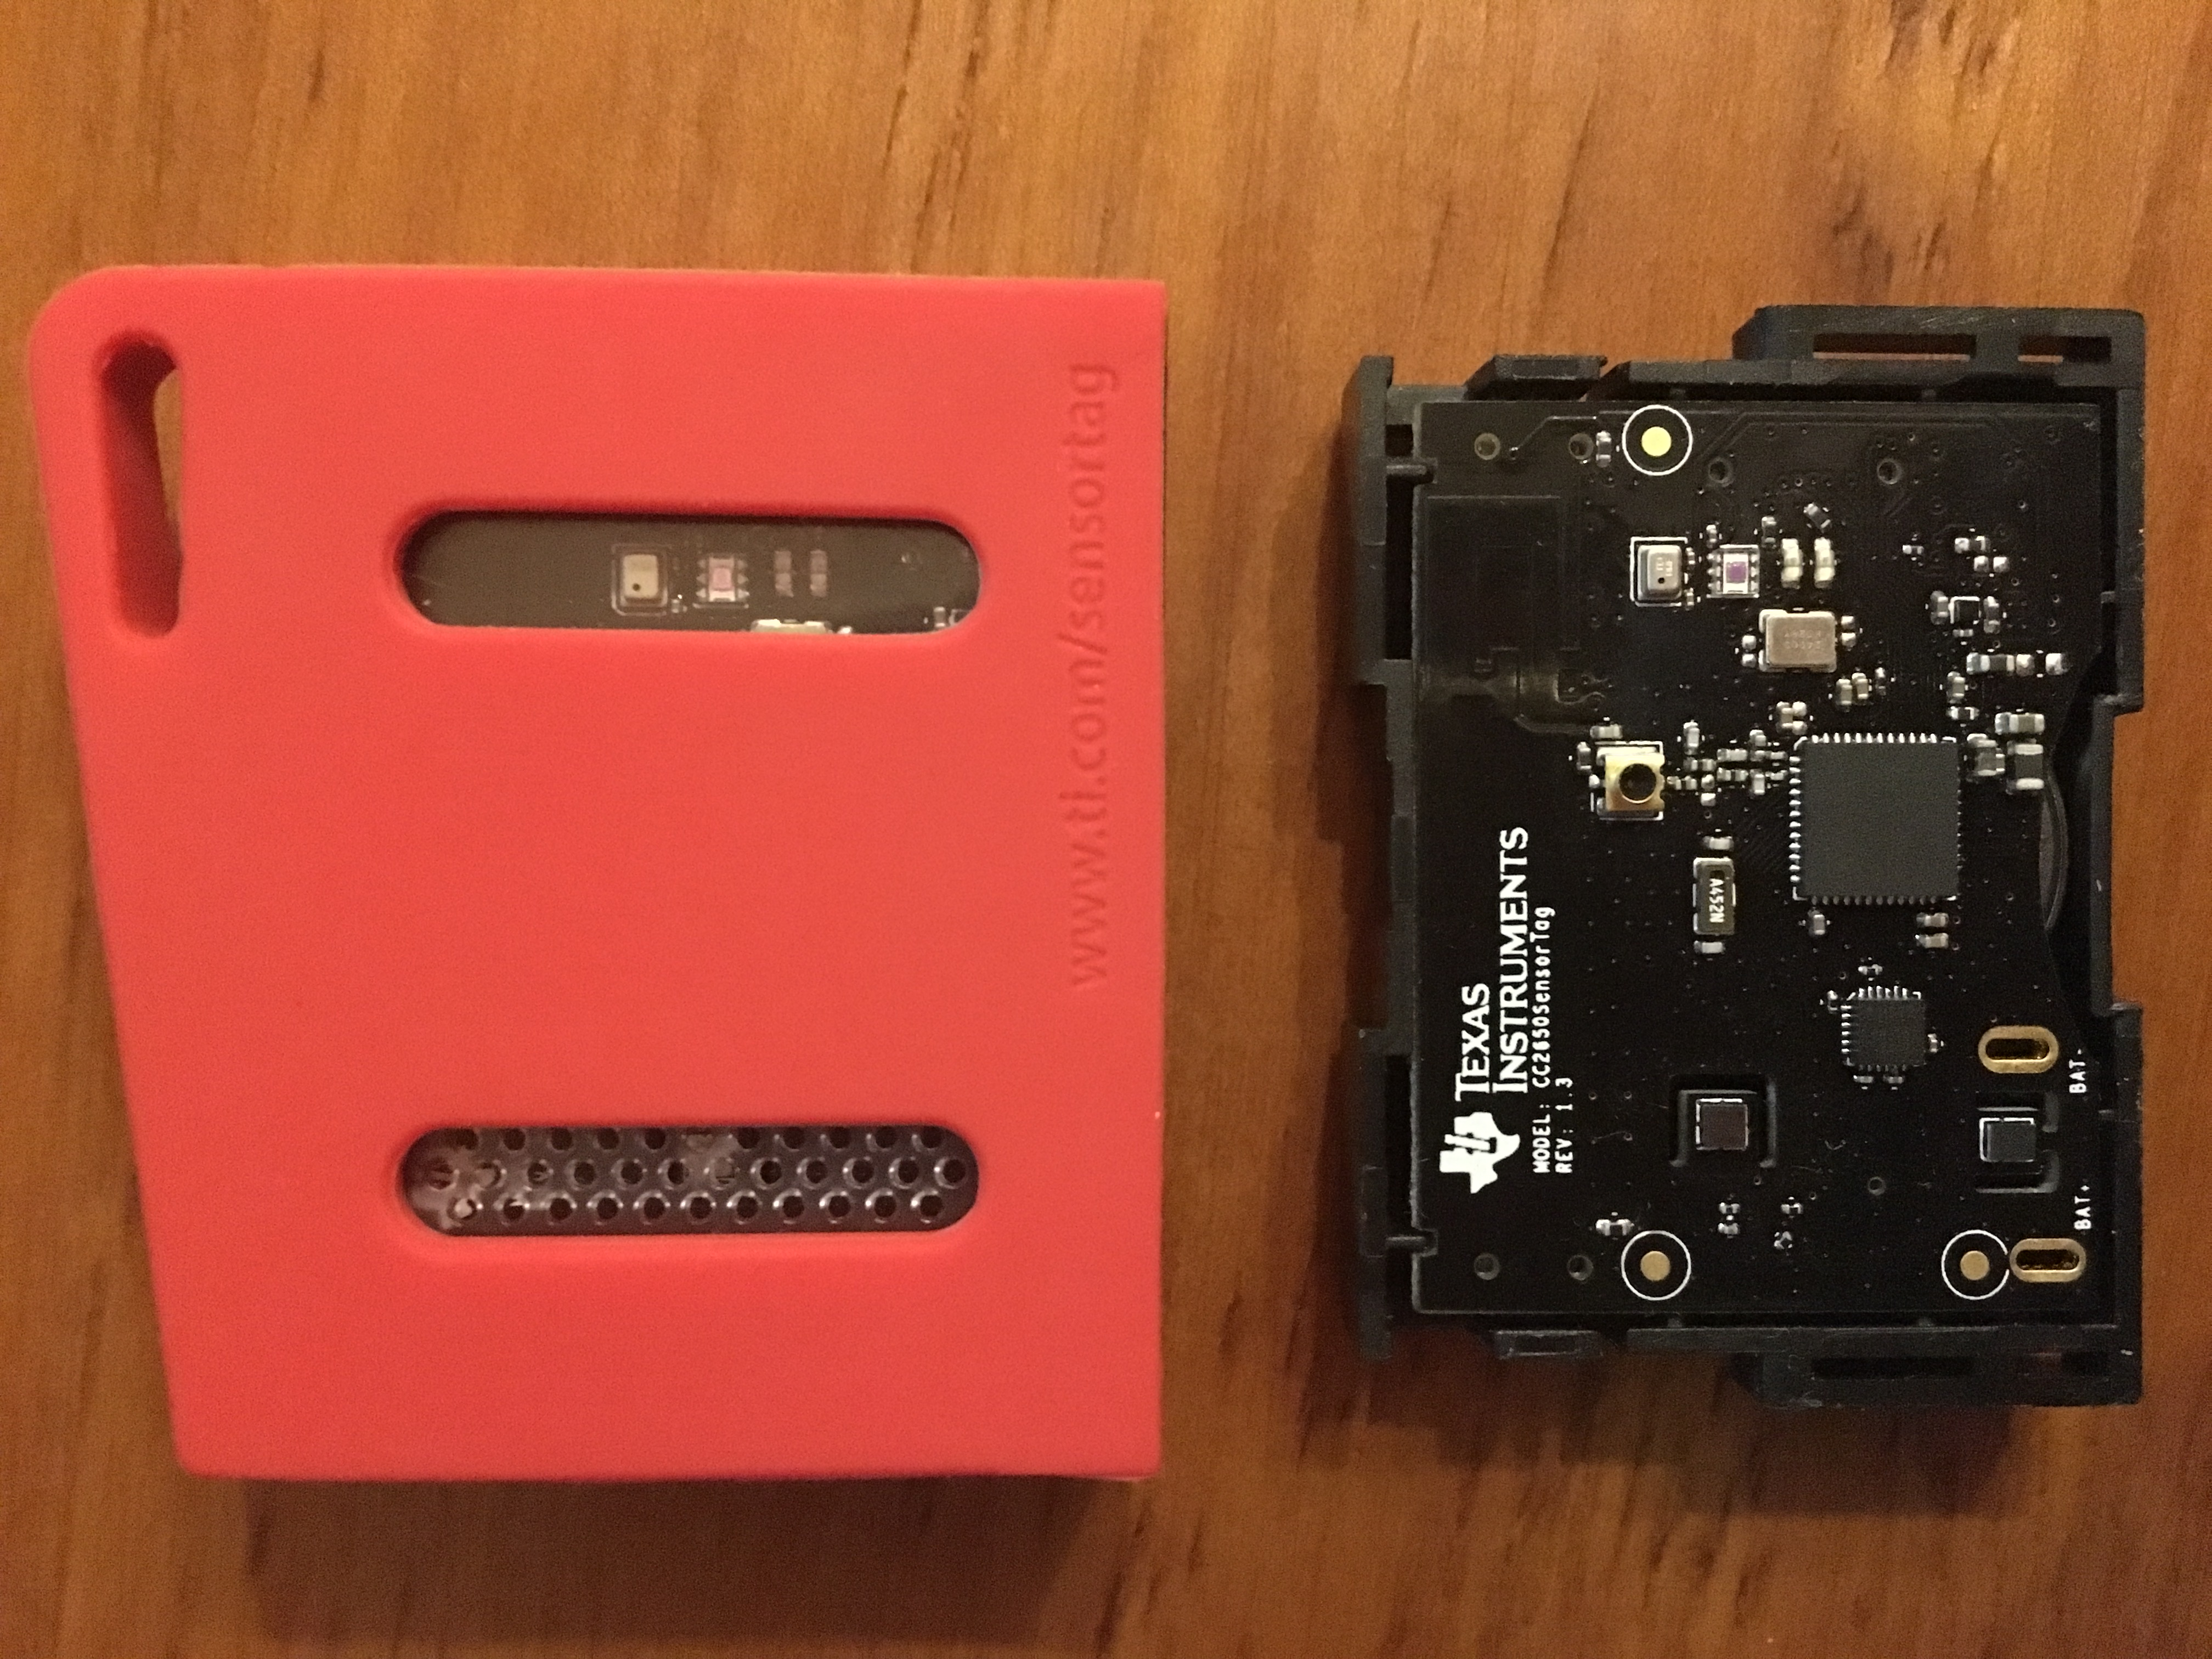
\includegraphics[width=0.5\linewidth]{4.Chapter/beacon.jpg}
	\caption[TI cc2650stk sensortag]{TI cc2650stk sensortag}
	\label{fig:beacon}
\end{figure}
